\documentclass[titlepage]{article}

\usepackage[utf8]{inputenc}
\usepackage[polish]{babel}
\usepackage{polski}
\usepackage{geometry}
\geometry{
    a4paper,
    margin=1in
}

\usepackage{amsmath,amssymb,amsthm,amsfonts}
\usepackage{lipsum}
\usepackage{hyperref}
\hypersetup{
pdftitle={Cybulski, Durkalec, Kurzyp - SmartCompass},
}
\usepackage{float}
\usepackage{placeins}
\usepackage{tabularx}
\usepackage{graphicx}
\usepackage{url}
\usepackage{listings}
\usepackage{color}
\usepackage{parskip}
\usepackage[counterclockwise]{rotating}
\graphicspath{ {./res/} }
% Headers and footers
\usepackage{fancyhdr, lastpage}
\pagestyle{fancy}
\lhead{PWr}
\chead{SmartCompass}
\rhead{Projekt Zespołowy, Lato 2024} 
% Footers
\lfoot{D. Cybulski, M. Durkalec, S. Kurzyp}
\cfoot{}
\rfoot{Strona \thepage \hspace{1pt} z \pageref{LastPage}}
\setlength{\headheight}{15pt}

% Custom footer and header on new chapter pages
\usepackage{etoolbox}
\patchcmd{\chapter}{\thispagestyle{plain}}{\thispagestyle{fancy}}{}{}

% Custom commands
% Display info about module
\newenvironment{module}[1]
{
    \begin{minipage}{\textwidth}
    \begin{equation*}
        #1
    \end{equation*}
    \begin{center}
    \renewcommand{\arraystretch}{1.2}
}
{
\end{center}
\end{minipage}
\vspace{1em}
\\ \noindent
}

\title{
SmartCompass \\ \vspace{5px}
\large Inteligentne urządzenie do nawigacji 
}
\author{
    \makebox[3.5cm]{Dominik Cybulski}  - \texttt{\href{mailto:255520@student.pwr.edu.pl}{255520@student.pwr.edu.pl}} \\
    \makebox[3.5cm]{Michał Durkalec}   - \texttt{\href{mailto:263917@student.pwr.edu.pl}{263917@student.pwr.edu.pl}} \\
    \makebox[3.5cm]{Stanisław Kurzyp}  - \texttt{\href{mailto:264477@student.pwr.edu.pl}{264477@student.pwr.edu.pl}}
}
\date{
\textbf{Prowadzący:} prof. Robert Burduk \\
Politechnika Wrocławska \\
Semestr letni 2024
}


\begin{document}

\maketitle

\tableofcontents

\part{Zarządzanie projektem}

\section{Założenia projektowe}
Celem projektu będzie zaprojektowanie i zbudowanie urządzenia służącego do nawigacji pieszej. Urządzenie będzie składało się z mikroprocesora z modułem Bluetooth, modułu GPS, wyświetlacza LCD oraz układu zasilającego. Konfiguracja będzie odbywała się za pomocą aplikacji mobilnej, w której możliwe będzie zaplanowanie trasy i wgranie jej do urządzenia.
Po skonfigurowaniu trasy, urządzenie będzie wskazywało kierunek i odległość do następnego punktu (na wyświetlaczu LCD).

\subsection{Wymagania projektowe}
Wymagania projektowe zostały określone za pomocą tablicy MoSCoW:

\begin{itemize}
    \item \textbf{Must have:}
          \begin{itemize}
              \item Urządzenie poprawnie wskazuje kierunek i odległość do kolejnych punktów trasy.
              \item Aplikacja pozwala na zaplanowanie trasy na mapie i wgranie jej do pamięci urządzenia.
              \item Po konfiguracji urządzenie działa autonomicznie, bez potrzeby komunikacji z aplikacją.
          \end{itemize}
    \item \textbf{Should have:}
          \begin{itemize}
              \item Bateria pozwala na całodzienne korzystanie z urządzenia (około 8 godzin).
              \item Urządzenie implementuje mechanizmy zmniejszające zużycie energii (np. wygaszanie ekranu).
              \item Aktualny stan nawigacji jest zapisywany w pamięci nieulotnej, co umożliwia wznowienie korzystania z urządzenia po utracie zasilania.
          \end{itemize}
    \item \textbf{Could have:}
          \begin{itemize}
              \item Urządzenie zapisuje aktualne położenie i pozwala na zgranie przebiegu trasy do aplikacji.
              \item Aplikacja wyświetla historię przebytych tras razem z czasami przejścia.
              \item Realizacja urządzenia na samodzielnie zaprojektowanej płytce PCB.
          \end{itemize}
    \item \textbf{Won't have:}
          \begin{itemize}
              \item Urządzenie nie posiada interaktywnego interfejsu użytkownika, wyświetla jedynie aktualny stan trasy.
          \end{itemize}
\end{itemize}

\section{Ryzyka projektowe}
Realizacja projektu wiąże się z kilkoma ryzykami, które zostały zidentyfikowane i ocenione pod względem prawdopodobieństwa wystąpienia oraz wpływu na projekt. Poniżej przedstawiono główne ryzyka oraz planowane działania w celu ich minimalizacji.

\subsection{Odejście członków zespołu}
\begin{itemize}
    \item \textbf{Prawdopodobieństwo:} Bardzo niskie
    \item \textbf{Wpływ:} Bardzo niski
    \item \textbf{Plan działania:} Akceptacja ryzyka ze względu na niskie prawdopodobieństwo i wpływ.
\end{itemize}

\subsection{Ograniczony budżet}
\begin{itemize}
    \item \textbf{Prawdopodobieństwo:} Średnie
    \item \textbf{Wpływ:} Wysokie
    \item \textbf{Plan działania:} Opracowanie szczegółowego kosztorysu oraz pozyskanie dodatkowych środków finansowych od Politechniki.
\end{itemize}

\subsection{Opóźnienia w dostawie komponentów}
\begin{itemize}
    \item \textbf{Prawdopodobieństwo:} Średnie
    \item \textbf{Wpływ:} Średnie
    \item \textbf{Plan działania:} Uwzględnienie potencjalnych opóźnień w harmonogramie realizacji oraz opracowanie alternatywnych planów montażu.
\end{itemize}

\subsection{Opóźnienia w montażu układu (PCB)}
\begin{itemize}
    \item \textbf{Prawdopodobieństwo:} Średnie
    \item \textbf{Wpływ:} Średnie
    \item \textbf{Plan działania:} Uwzględnienie potencjalnych opóźnień w harmonogramie realizacji oraz opracowanie alternatywnego planu montażu.
\end{itemize}

\subsection{Niewystarczające umiejętności}
\begin{itemize}
    \item \textbf{Prawdopodobieństwo:} Średnie
    \item \textbf{Wpływ:} Średnie
    \item \textbf{Plan działania:} Akceptacja ryzyka oraz regularne szkolenia i konsultacje w zespole.
\end{itemize}

\subsection{Skomplikowana dokumentacja techniczna komponentów}
\begin{itemize}
    \item \textbf{Prawdopodobieństwo:} Średnie
    \item \textbf{Wpływ:} Niskie
    \item \textbf{Plan działania:} Wybór innych komponentów lub korzystanie z nieoficjalnych dokumentacji i wsparcia społeczności online.
\end{itemize}

\section{Harmonogram projektu}
Projekt został podzielony na trzy główne etapy:

\begin{itemize}
    \item \textbf{Etap I - Projektowanie} (do 8 kwietnia 2024)
          \begin{itemize}
              \item Opracowanie listy komponentów elektronicznych.
              \item Analiza i wybór komponentów.
              \item Projekt układu elektronicznego.
              \item Wybór technologii programowania aplikacji mobilnej.
              \item Projektowanie widoków aplikacji mobilnej.
              \item Opracowanie protokołu komunikacji między urządzeniem a aplikacją.
          \end{itemize}
    \item \textbf{Etap II - Prototypowanie i testowanie} (do 6 maja 2024)
          \begin{itemize}
              \item Zakup komponentów.
              \item Montaż układu na płytce prototypowej.
              \item Programowanie urządzenia i aplikacji mobilnej.
              \item Testy komunikacji między aplikacją a urządzeniem.
          \end{itemize}
    \item \textbf{Etap III - Montaż} (do 27 maja 2024)
          \begin{itemize}
              \item Montaż układu w wybranej technologii.
              \item Budowa obudowy urządzenia.
              \item Przygotowanie wersji produkcyjnej aplikacji mobilnej.
          \end{itemize}
\end{itemize}

\section{Zarządzanie zespołem}
\subsection{Podział zadań}
Przed rozpoczęciem projektu został ustalony następujący podział zadań:
\begin{itemize}
    \item \textbf{Dominik Cybulski, Michał Durkalec:} \\ Projektowanie układu elektronicznego, programowanie urządzenia.
    \item \textbf{Stanisław Kurzyp:} \\ Projektowanie aplikacji mobilnej.
\end{itemize}

\subsection{Planowanie pracy}
Do planowania poszczególnych zadań oraz monitorowania postępów wykorzystane zostało narzędzie Github Projects \cite{github-projects-docs}, które pozwala na
\begin{itemize}
    \item Tworzenie zadań i przypisywanie ich do członków zespołu.
    \item Planowanie terminów realizacji zadań.
    \item Monitorowanie postępów prac.
    \item Łączenie zadań z konkretnymi gałęziami kodu w systemie kontroli wersji.
\end{itemize}
\part{Implementacja}

\section{Projekt urządzenia}
\subsection{Napotkane problemy}
Tu można opisać problemy napotkane podczas projektowania urządzenia.

\section{Firmware}
\subsection{Napotkane problemy}
Tu można opisać problemy napotkane podczas pisania oprogramowania.

\section{Aplikacja mobilna}
\subsection{Napotkane problemy}
Tu można opisać problemy napotkane podczas pisania oprogramowania.
\part{Efekty}

\section{Prototyp urządzenia}

\section{Aplikacja mobilna}
\subsection{Widoki aplikacji}
\subsubsection{BLE connection}

\begin{figure}[H]
    \centering
    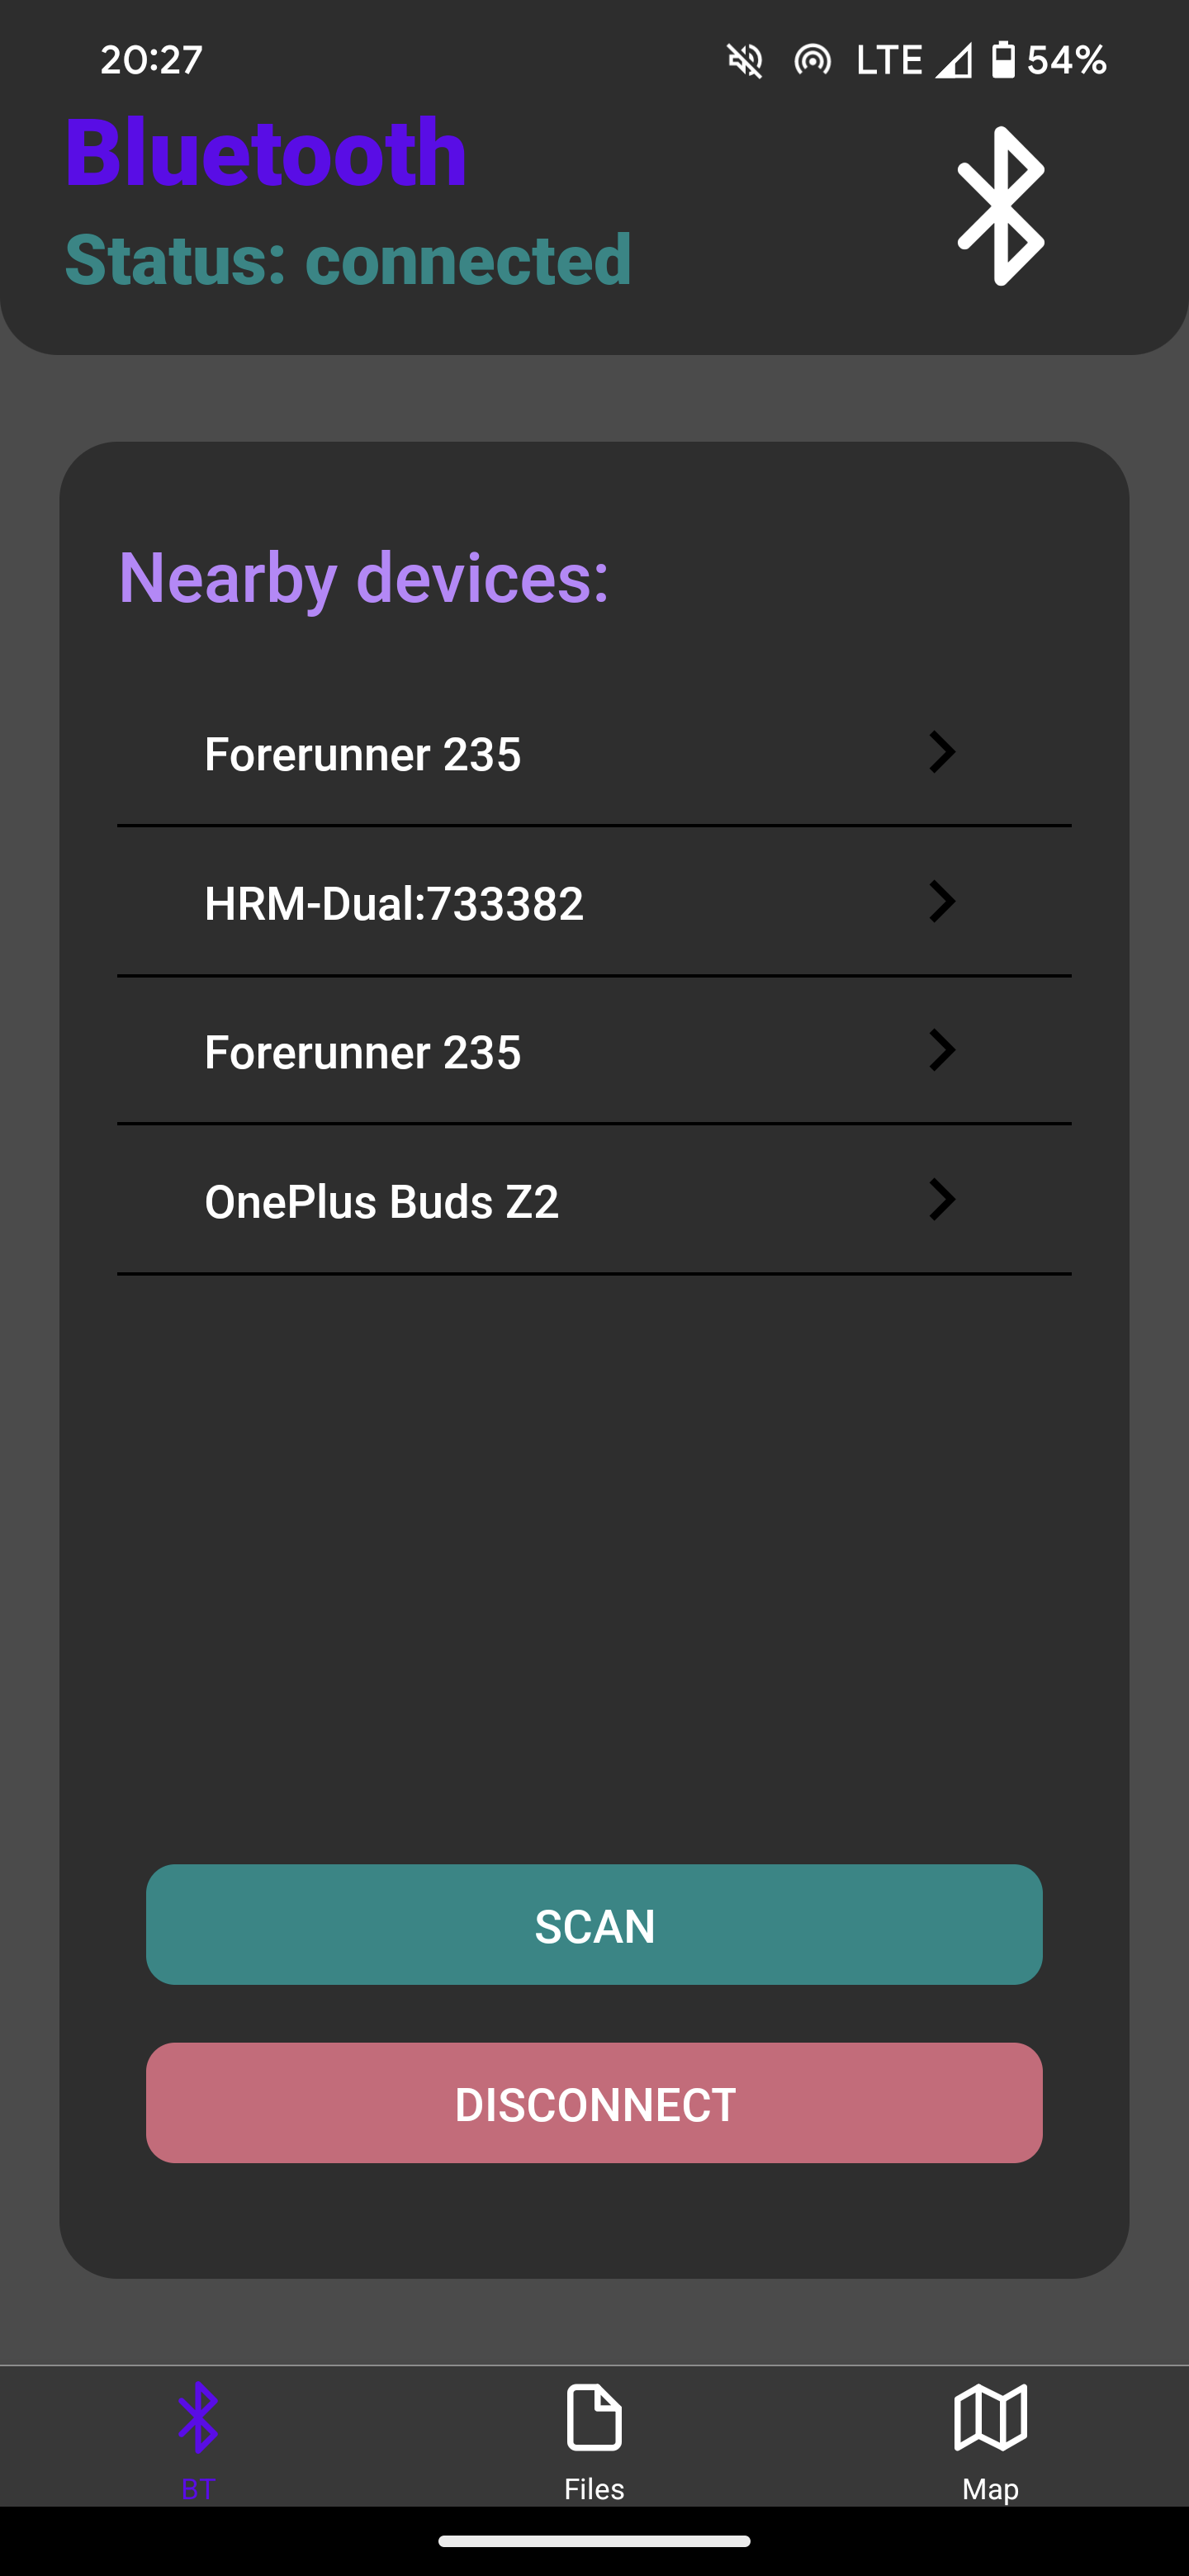
\includegraphics[scale = 0.07]{res/BT.png}
    \caption{Ekran BLE connection}
\end{figure}

Widok ten pozwala użytkownikowi rozpocząć skanowanie pobliskich urządzeń BLE, a następnie wybrać jedno z nich i połączyć się z nim. Jeśli jest to urządzenie SmartCompass, to znaleziony zostanie udostępniany przez nie serwis BLE, którego UUID zapisane jest w aplikacji. Nawiązanie z nim połączenia umożliwi przesyłanie do tego urządzenia danych.
Na ekranie tym znajdują się również dwa przyciski:
\begin{itemize}
    \item \textbf{Przycisk Scan} - rozpoczyna skanowanie urządzeń
    \item \textbf{Przycisk Disconnect} - rozłącza z urządzeniem.
\end{itemize}

\subsubsection{Files}
\begin{figure}[H]
    \centering
    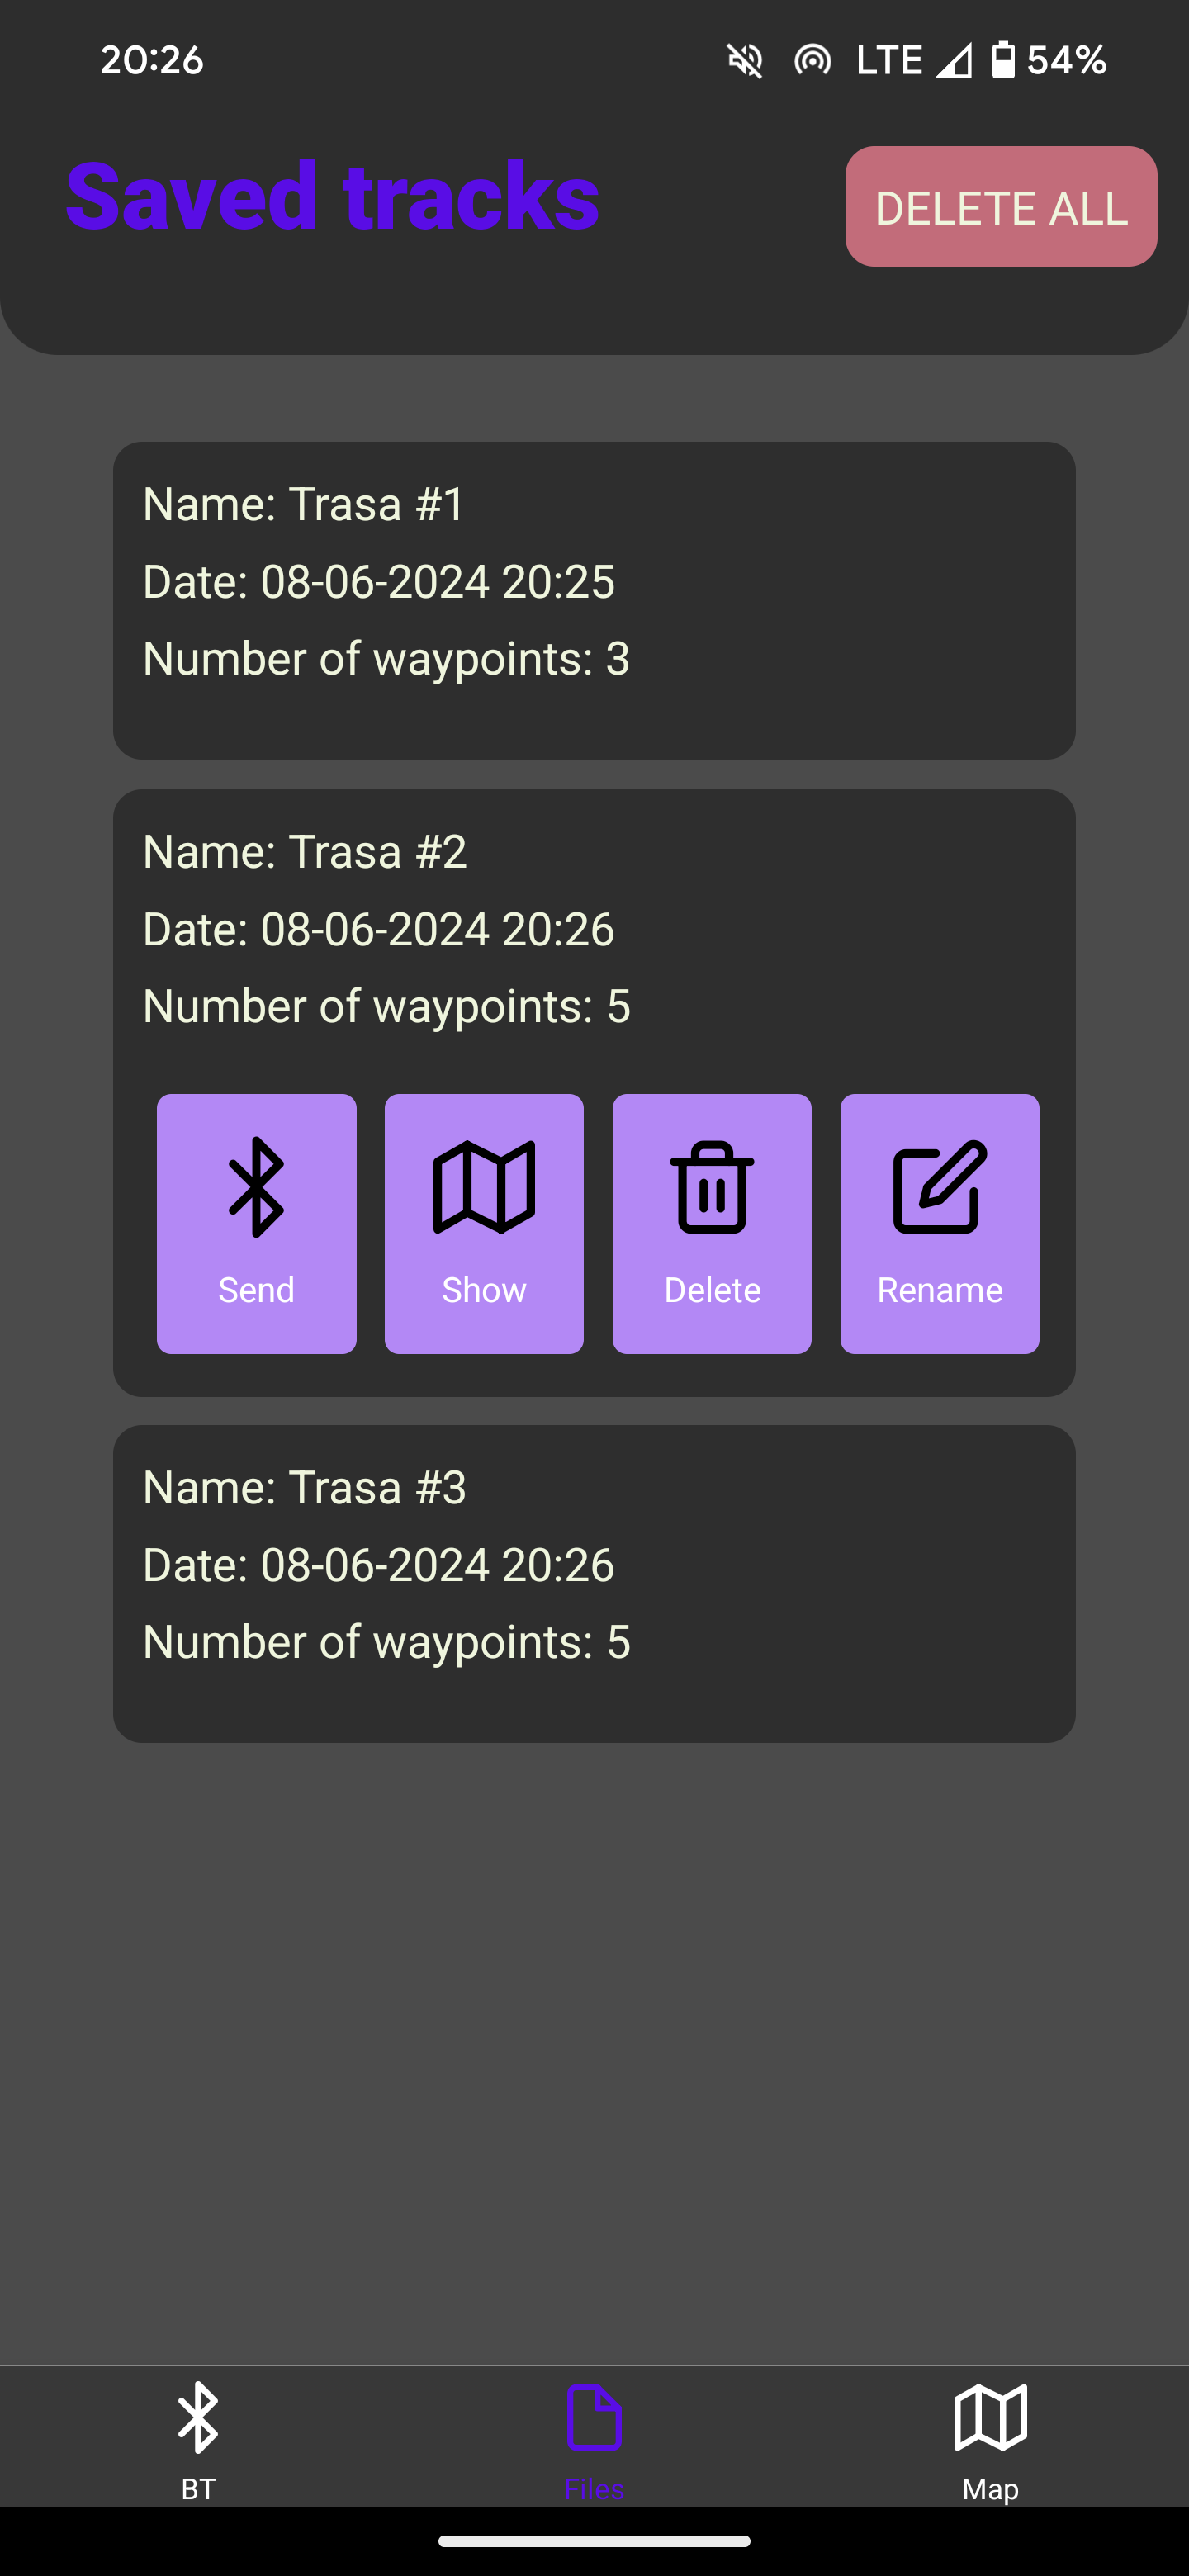
\includegraphics[scale = 0.07]{res/Files.png}
    \caption{Ekran plików}
\end{figure}

Widok ten oferuje możliwość przeglądania zapisanych w urządzeniu tras

Po kliknięciu w trasę, rozwinie się menu z 4 przyciskami:
\begin{itemize}
    \item \textbf{delete} – usuwa wybraną trasę.
    \item \textbf{edit} – przenosi do widoku mapy i wyświetla w nim wybraną trasę pozwalając na jej edycję.
    \item \textbf{send} – pozwala przesłać wybraną trasę do urządzenia SmartCompass jeśli jest ono połączone.
\end{itemize}

\subsubsection{Map}
\begin{figure}[H]
    \centering
    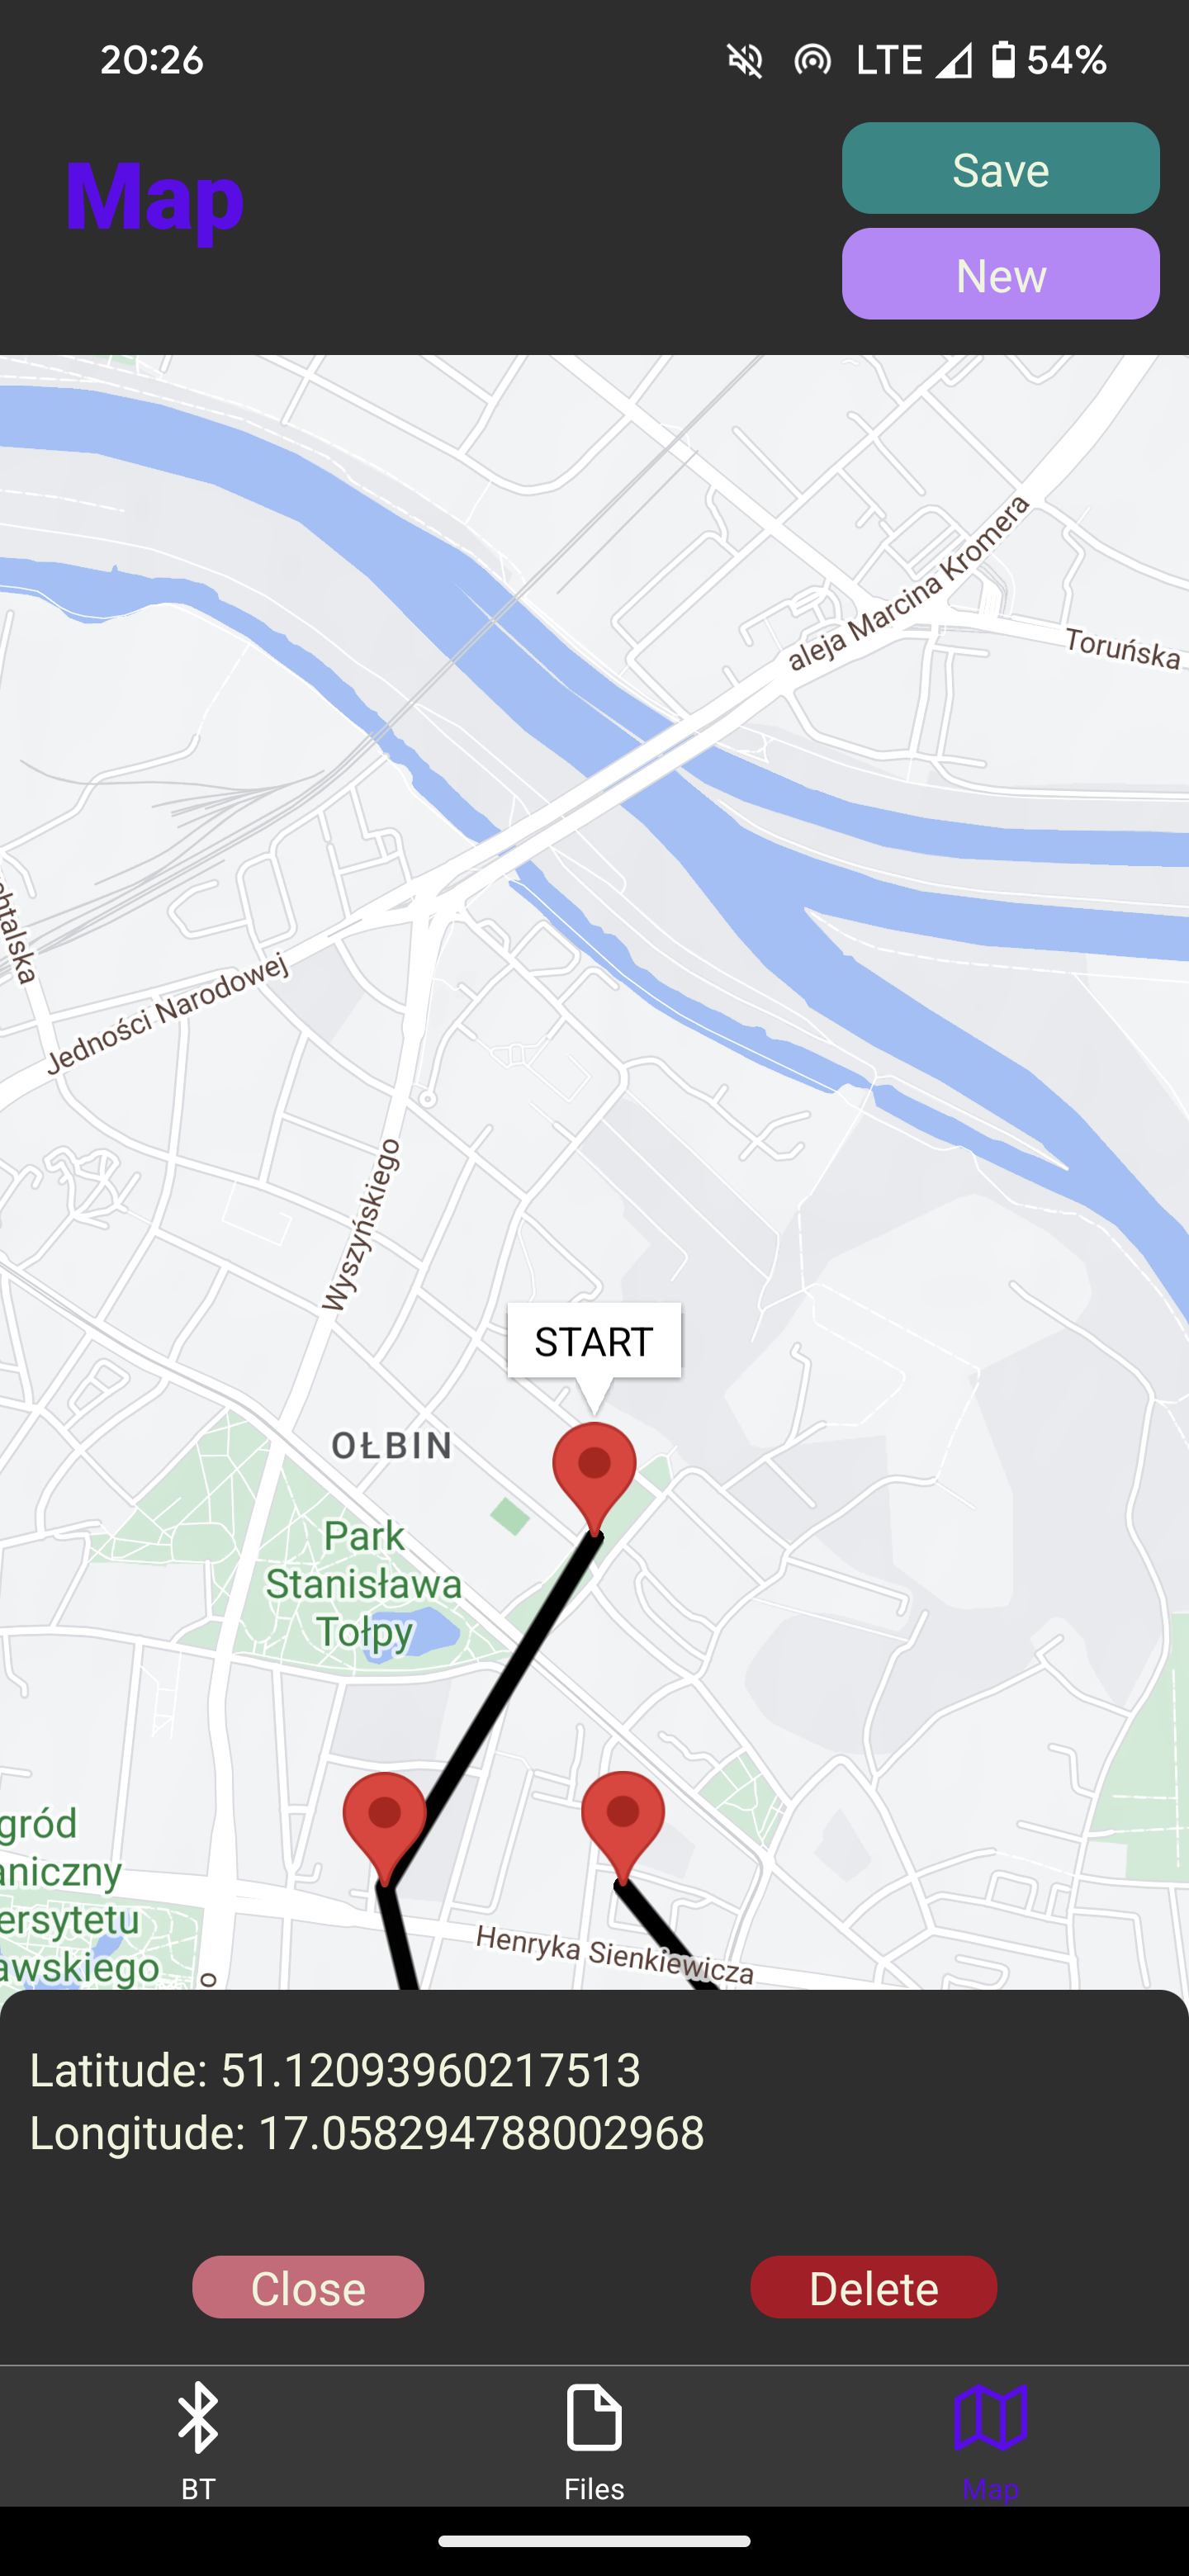
\includegraphics[scale = 0.07]{res/Map.png}
    \caption{Ekran Mapy}
\end{figure}
Widok mapy oferuje możliwość rysowania trasy, dodawania nowej trasy oraz zapisu obecnie narysowanej trasy. W tym celu wykorzystywane są poniższe przyciski:

\begin{itemize}
    \item \textbf{NEW} – wyczyszczenie punktów na mapie, jeśli trasa jest zapisana nie zostanie ona utracona. Pozwala na rysowanie nowej trasy
    \item \textbf{SAVE} – służy do zapisu aktualnie narysowanej trasy. Po kliknięciu pojawi się okienko z miejscem na wpisanie nazwy trasy. Trasa zapisana zostanie do wewnętrznej, statycznej pamięci urządzenia i widoczna będzie w widoku \textbf{Files} po restarcie aplikacji.
\end{itemize}
Ponadto do interakcji z mapą użytkownik wykorzystuje następujące gesty:
\begin{itemize}
    \item \textbf{przytrzymanie palcem w pustym miejscu na mapie} – dodanie nowego punktu
    \item \textbf{dłuższe przytrzymanie znacznika punktu} – przejście w tryb przenoszenia punktu poprzez przesuwanie palcem po ekranie. Znacznik zostanie upuszczony po oderwaniu palca od ekranu
    \item \textbf{kliknięcie w znacznik} – nad znacznikiem wyświetli się małe pole z jego numerem na trasie lub napisem \textit{START/META}. Ponadto na dole ekranu wyświetli się okno z dokładną lokalizacją punktu. Kliknięcie w puste miejsce na mapie spowoduje zamknięcie tego okna i zniknięcie pola nad znacznikiem.
\end{itemize}

\section{Możliwości rozwoju}

\subsection{Rozwój aplikacji mobilnej}
Aplikacja realizuje zdefiniowane dla niej założenia. Potencjał na rozwój znajduje się w interfejsie użytkownika i, pomimo że jest kompletny, można wprowadzić zmiany, które poprawią ogólne wrażenia oraz intuicyjność korzystania z aplikacji dla użytkownika końcowego.

\bibliographystyle{plain}
\bibliography{refs}

\end{document}